\documentclass[a4paper,12pt]{article}
\usepackage{graphicx}
\usepackage[a4paper]{geometry}
\usepackage{fancyhdr}
\pagestyle{fancy}
\usepackage{array}
\usepackage{apacite}
\usepackage{mathptmx}
\usepackage{enumerate}

\title{\textbf{OPINION MINING ON SOCIAL MEDIA DATA}}
\author{
\textbf{TAN CHONG RAEN 1121115725}\\Faculty of Computer Information, \\Student of Multimedia University, \\Cyberjaya, Malaysia.\\ Email: \url{chongraentan@gmail.com}
} 
\break
\date{\today}

\begin{document}
\thispagestyle{empty}
\newgeometry{top=1mm,left=2cm}
\begin{center}
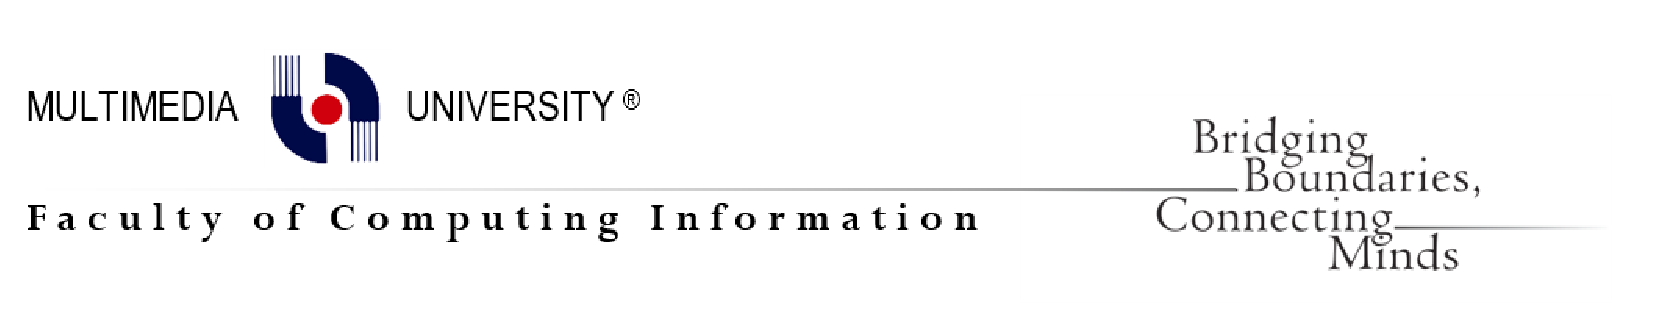
\includegraphics[width=18cm]{mmu.eps}
\break\break\break\break
\Huge
TPT 1201\break\break
RESEARCH METHODOLOGY \break
IN \break
COMPUTER SCIENCE \break\break\break\break
\textless ASSIGNMENT 2\textgreater \break\break\break\break 
\Large
PREPARE BY \break\break
\begin{tabular}{| m{7.5cm} | m{9cm} |}
\hline
\hspace{2.3cm}Student ID &\hspace{2.5cm}Student Name \\
\hline
\hspace{2.05cm}1121115725 &\hspace{1.5cm} TAN CHONG RAEN \\
\hline
\end{tabular}
\break\break
LECTURE SECTION \hspace{5mm}: TC01\break
TUTORIAL SECTION \hspace{2mm}: TT02\break
LECTURER: \textit{DR. POO KUAN HOONG}
\end{center}

\bibliographystyle{apacite}
\lhead{Tan Chong Raen 1121115725}
\rhead{TPT 1201}

\restoregeometry
\maketitle
\newpage
\thispagestyle{empty}
\tableofcontents
\thispagestyle{empty}

\linespread{1.5}
\newpage
\setcounter{page}{1}
\section{Executive Summary of Research Proposal} 
\hspace*{1cm}Social media has become a very popular micro-blogging platform which play as a communication tool among Internet users. It allows users to share or post their opinions on the platform with their mobile devices or computers. Therefore, there are a massive of textual information being generated. All of these data may help company managers or businessman to make an informed decisions. So, it is worthwhile research for analyze and found the valuable and meaningful information from these data. However, there are few problems that we challenged. As post of the micro-blog usually is short and informal. Moreover, the existing algorithms are not fit in type of text and it make the accuracy of mining become lower. So, we proposed a system architecture called  \textit{Opinion Miner} to analyze the sentiments of textual information automatically and combine the social media data with the system to do the sentiment analysis and improve the accuracy. For the algorithm of  \textit{Opinion Miner}, we distribute into four steps. There are \textit{preprocessing, extracting, short text classifying, and training multiple classifiers}. Finally, the result of experiment as our expectation as the accuracy of the  \textit{Opinion Miner} is works better than the existing algorithm,  \textit{Unigram Model}, which accuracy is 67.58\% compare to 70.39\%.
\section{Introduction}
\hspace{1cm}Nowadays, social media has become a marketing tool and being actively used by governments, people, organizations and institutions. It provide a micro-blogging platform to every internet users to share their opinion, diary of their life, or they can discuss about the main issues with each other. Not only that, some organizations or users also used the social media for e-commerce purpose. They allows their customers to do product reviews, purchase products, or even private message them to get the customer services. Therefore, we can realize that the power of the social media and its data can be help the organizations or users to keep track the customer opinions by using a sentiments analysis system to analyze the sentiment content of the reviews. 
Opinion is the term that can help people to make a better decision. For example, governments collects feedback that provide by its people and analyze it for getting the rating of the policies. However, the post of the microblogging user is short and informal. So it make the existing algorithm could not working well. And the accuracy of analysis system is important since it may affect the users during the decision making process. For these reasons, we purposed the new system architecture which called \textit{Opinion Miner}.
\textit{Opinion Miner} is a system that help to improve the accuracy of the sentiment analysis. Moreover, this system able to do \textit{Short Text Classification} and the machine would learn how to extract the social media data that contain opinion and train them in the distinct categories (i.e. positive, negative). The idea for implement this system is to apply the domain-specific training data and develop a generic classification model with social media data.
\section{Justification of Research}
\hspace*{1cm}The purpose of this empirical research is to analyze the social media data and generate the useful information to help the users or mangers to make an informed decision. Furthermore, we proposed a system called \textit{Opinion Miner} to improve the accuracy of the existing opinion mining algorithm. \textit{Opinion Miner} is a system architecture that used to distribute the positive or negative opinion in the social media data. So if the experiment shows the higher accuracy result then it may help the managers or users to make better decisions.
\section{Research Objectives}
\begin{itemize}
\item To implement a system that able to do the sentiment analysis from social media data.
\item To improve the accuracy of sentiment analysis on social media data.
\end{itemize}
\section{Literature Review}
\hspace{1cm}According to the one of research paper that we reviewed\cite{APPP2010}. They stated in that paper where there are few model provided to build the sentiment classifier such as \textit{Naïve Bayes, Conditional Random Fields, and Support Vector Machine\cite{Pang2002}}. According their research, Naïve Bayes yielded the best result. In additional, Naïve Bayes classifier is following the Bayes’ theory. Furthermore, they introduce two strategies to increasing the accuracy of sentiment analysis. First strategy is depend on formula Shannon entropy and the second strategy is apply the formula of salience. In their experiments, the result indicates that the accuracy of salience is higher than entropy. Besides that, we also review another research paper about the \textit{Sentiment analysis of twitter data}\cite{SentAnaly2011}. In their research, they tested for two-way classification task and three-way classification task. And they apply five different models to each task. The models that they apply are \textit{Unigram, Senti-features, Kernel, combination of Unigram and Senti-features, and combination of Kernel and Senti-features}. During their experiment, the result shows that the accuracy of combination of Unigram and Senti-features is the highest in two-way classification task but the result shows in the three-way classification task that the accuracy of combination of Kernel and Senti-features is the highest. According to these two research paper, we found that the accuracy of the sentiment analysis may decrease significantly when apply the Unigram model in n-way classification task (when n \textgreater =3). Furthermore, the formula of salience would help to increase accuracy of the sentiment analysis. 
\section{Research Methodology}
\hspace{1cm}In this research, we need to combine data of Twitter, one of the most popular social media, with our system for do the sentiment analysis and build a manually labeled data as the training data \cite{XBP2008} in our model. After all prepared statement is done, we fetch the tweets from Twitter, and perform the first step in our system architecture, \textit{Preprocessing}, to pre-process all the tweets. In this process, our system transformed all the words of tweet into lower case and eliminating whether the tweets are English, less than five words after greeting words, or just a URL. Moreover, this system detect all the words that start with “\@” and replaced them with “USER” since “\@” is represent a user in Twitter. In additional, this system convert repeated characters to a character such as “sooooooooo” covert to “so”.  After that, we apply a tool \textit{Tree Tagger} in our system to provide a \textit{Part-Of-Speech} tag to every word in text. In the following step, we apply \textit{Naïve Bayes (NB) classifier} on the training data to classify whether the tweets is the group of opinion or non-opinion. And its formula is shows in the equation(1).\linebreak \linebreak
\begin{equation}
P(tk|c) = \frac{T_{ct}+1}{\sum_{t}(T_{ct}+1)}
\end{equation} \linebreak \par
Next is the Short Text Classification, we apply two different algorithm during this step. There are Mutual Information (MI)\cite{Susan1998} and $X^2$ Feature Selection ($X^2$). For the formula of MI is state in equation(2) where for each class C and each feature F, there is a score to measure how much F can contribute to making a correct decision on class C.\linebreak \linebreak
\begin{equation}
MI(C;F) = \sum_{}\sum_{}P(C,F)log\frac{P(C,F)}{P(C)P(F)}
\end{equation}\linebreak \par
In the other hand, the formula of $X^2$ is declare in the equation(3) where N is the total number of training sentences. N11 is the number of co-occurrences of the feature F and the class C. N10 is the number of sentences containing the feature F but that are not in class C. N01 is the number of sentences in class C that do not contain feature F. N00 is the number of sentences not in C and that do not contain feature F.\linebreak \linebreak
\begin{equation}
X^2(F,C) = \frac{N(N11-N00-N10N01)^2}{(N11+N01)(N11+N10)(N10+N00)(N10+N00)}
\end{equation}\linebreak \par
After complete the classification of short text, this system train the classifiers in the distinct categories with different training data that we labeled manually before.Furthermore, we develop many binary classifiers with all of the training data and Naïve Bayes algorithm for this system.\par
Finally, we can start to evaluate the system and shows the result to predict the semantic orientations on Twitter. Now, we distribute the experiments into three parts. First is prepare the data sets. Next is experimental result of each step and the last is the comparison between existing model and Opinion Miner. For the first part, we have prepared two data sets that are Training Data and Testing Data. In additional, our data is collected from Twitter with Twitter API and we set the language of the data is English. Moreover, we only crawl tweet of three different categories from Twitter that are Movie, Camera, and Mobile Phone.
\par Next, this system extract the tweets that are contain opinion and filter out all the non-opinion tweets. After extracted the tweets, we will process to \textit{Short Text Classification}. During this process, we apply two different feature selection to classify the text, which are Mutual Information and $X^2$ Feature Selection, and the top N features with highest accuracy will be apply for the features set to do the test. After that, we determine the semantic analysis of tweet by using a model of Naive Bayes.
\par Last but not least, we will show the result of Opinion Miner and existing model and compare them in a table.
\begin{center}
TABLE I : RESULT OF OPINION MINER 
\linebreak \linebreak
\begin{tabular}{|c|c|c|c|}
\hline
& Positive (318) & Negative (66) & Non-opinion (126) \\
\hline
Positive (318) & 282 & 28 & 64  \\
\hline
Negative (66) & 15 & 21 & 6 \\
\hline
Non-opinion (126) & 21 & 17 & 56 \\ 
\hline
\end{tabular}
\linebreak \linebreak \linebreak
\par TABLE II : RESULT OF UNIGRAM MODEL 
\linebreak \linebreak
\begin{tabular}{|c|c|c|c|}
\hline
& Positive (318) & Negative (66) & Non-opinion (126) \\
\hline
Positive (318) & 250 & 19 & 59  \\
\hline
Negative (66) & 20 & 40 & 13 \\
\hline
Non-opinion (126) & 48 & 7 & 54 \\ 
\hline
\end{tabular}
\linebreak \linebreak \linebreak
\par TABLE III : ACCURACY OF RESULT 
\linebreak \linebreak
\begin{tabular}{|c|c|}
\hline
& Accuracy\\
\hline
Opinion Miner & 70.39\%  \\
\hline
Unigram & 67.58\% \\
\hline
\end{tabular}
\end{center}

\newpage
\bibliography{MyBib}{}
\newpage

\begin{flushleft}
\textbf{Project Assessment: }
\\
\begin{tabular}{|m{60mm} | m{90mm} |}
\hline
Title of your research projec & OPINION MINING ON SOCIAL MEDIA DATA \\
\hline
Member of your project & TAN CHONG RAEN\\
\hline
Executive Summary (5 marks) & \\
\hline
Introduction (3 marks)& \\
\hline
Justification of Research (3 marks) & \\
\hline
Research Objectives (3 marks)& \\
\hline
Literature Review  (6 marks)& \\
\hline
Research Methodology  (8 marks) & \\
\hline
References (2 marks)& \\
\hline
\end{tabular}
\end{flushleft}
\end{document}
